\documentclass[answers]{exam}
% 'texPreamble' contains formatting and macros. 
% https://github.com/pwesterbaan/scripts/tree/master/texmf/tex/latex/local
\usepackage{texPreamble}
\hypersetup{hidelinks}
\usepackage{relsize}
\usepackage{tkz-euclide}
\usepackage[titles]{tocloft}
\renewcommand{\cftsecleader}{\cftdotfill{\cftdotsep}}
\usetkzobj{all}
%% Externalize graphics and save in ./images/ folder
%% pdflatex -shell-escape <tex file>
%% The document can be compiled with the two following
%% lines commented out, but will recompile all figures
%% each time.
\usetikzlibrary{external}
\tikzexternalize[prefix=images/]
%% Uncomment the following line to recompile ALL images
%    \tikzset{external/force remake}
%% Place this line in braces around the image to recompile
%% e.g. { tikzset{...} \begin{tikzpicture} ... \end{tikzpicture} }
%% 
\usepackage{tabularx}
\extraheadheight{0.25in}
\extrafootheight{1.0in}
\extrawidth{1in}
% ----------------------------------------------------------------
\makeatletter
\title{Math 1060 Class notes\\[0.25\baselineskip]Spring 2020}
\author{\thefname\ \thelname}

\pagestyle{headandfoot}

%\firstpageheader{\@title\\\@date}{}{Math 1060}
%\firstpageheadrule

\newcommand*{\currentname}{\@currentlabelname}

\runningfootrule
\runningfooter{\parbox{0.45\linewidth}{\currentname}}{\thepage}{\@title}
\makeatother

\begin{document}
   %% Title
  \pagenumbering{roman}
  \vspace*{\stretch{1}}
  \begin{center}
    \makeatletter
    {\huge
    \@title}\\[\baselineskip]
    \@author\\[\baselineskip]
    Last updated:
    \@date\\
    \makeatother
  \end{center}
  \vspace*{\stretch{1}}
  \thispagestyle{empty}
  \pagebreak
  \pagestyle{headandfoot}

  \renewcommand{\contentsname}{Table Of Contents}
  \renewcommand\thesection{}
  \tableofcontents
  \newpage
  
  \makeatletter
  \firstpageheader{}{}{}
  \firstpagefooter{\parbox{0.45\linewidth}{\currentname}}{\thepage}{\@title}
  \firstpagefootrule
  \makeatother
  \pagenumbering{arabic}
  \setcounter{page}{1}
  %% everything else
  \relscale{1.4}

\input{briggs1_03}
\input{briggs1_04}
\input{briggs2_01}
\input{briggs2_02}
\documentclass[answers]{exam}
\usepackage{texPreamble}
\usepackage{relsize}
\usepackage{tabularx}
\extraheadheight{0.25in}
\extrafootheight{1.0in}
\extrawidth{1in}
% ----------------------------------------------------------------

\begin{document}
  \section{2.3: Techniques for Computing Limits}
    \begin{ex*}\ 
    
      \begin{tasks}(2)
        \task $\ds\lim_{x\to 3} \frac{1}{2}x-7$
        \task $\ds\lim_{x\to 2} 6$
      \end{tasks}
      \vspace*{\stretch{1}}
    \end{ex*}
    \begin{defn*}[Briggs]
      \textbf{Limit Laws:} Assume $\ds\lim_{x\to a} f(x)$ and $\ds\lim_{x\to a} g(x)$ exist. The following properties hold, where $c$ is a real number, and $n>0$ is an integer.
      
    \begin{center}
      \def\arraystretch{2.5}
      \begin{tabular}{llL}
        1.&\textbf{Sum:}
          &\ds\lim_{x\to a}\parens{f(x)+g(x)}=\lim_{x\to a}f(x)+\lim_{x\to a}g(x)\\
        2.&\textbf{Difference:}
          &\ds\lim_{x\to a}\parens{f(x)-g(x)}=\lim_{x\to a}f(x)-\lim_{x\to a}g(x)\\
        3.&\textbf{Constant multiple:}
          &\ds\lim_{x\to a}{cf(x)}=c\lim_{x\to a}f(x)\\
        4.&\textbf{Product:}
          &\ds\lim_{x\to a}{f(x)g(x)}=\parens{\lim_{x\to a}f(x)}\parens{\lim_{x\to a}g(x)}\\
        5.&\textbf{Quotient:}
          &\ds\lim_{x\to a}{\frac{f(x)}{g(x)}}=\frac{\lim_{x\to a}f(x)}{\lim_{x\to a}g(x)}, \text{ provided} \lim_{x\to a} g(x)\neq 0\\
        6.&\textbf{Power:}
          &\lim_{x\to a}\parens{f(x)}^n=\parens{\lim_{x\to a}f(x)}^n\\
        7.&\textbf{Root:}
          & \lim_{x\to a}\parens{f(x)}^{\sfrac{1}{n}}=\parens{\lim_{x\to a} f(x)}^{\sfrac{1}{n}}
       \end{tabular}
     \end{center}
    \end{defn*}
    \pagebreak
    \begin{ex*}
      Suppose $\ds \lim_{x\to 2} f(x)=4, \lim_{x\to 2} g(x)=5$ and $\ds\lim_{x\to 2}h(x)=8$. 
      \begin{tasks}(1)
        \task $\ds\lim_{x\to 2} \frac{f(x)-g(x)}{h(x)}$\\[15pt]
        \task $\ds\lim_{x\to 2} \parens{6f(x)g(x)+h(x)}$\\[15pt]
        \task $\ds\lim_{x\to 2} \parens{g(x)}^3$
      \end{tasks}
      \vspace*{\stretch{1}}
    \end{ex*}
    \begin{ex*}
      For $g(x)=\dfrac{x+6}{x^2-36}$, find
      \begin{enumerate}
        \item $\ds\lim_{x\to 0} g(x)$\\[25pt]
        \item $\ds\lim_{x\to -6} g(x)$
      \end{enumerate}
      \vspace*{\stretch{1}}
    \end{ex*}
    \pagebreak
    \begin{ex*}
      $\ds\lim_{x\to 2} \frac{\sqrt{2x^3+9}+3x-1}{4x+1}$
      \vspace*{\stretch{1}}
    \end{ex*}
    \begin{ex*}
      $\ds\lim_{x\to 1} f(x)$ where $f(x)=\begin{cases}
        -2x+4& \text{if }x\leq 1\\
        \sqrt{x-1}& \text{if } x>1
      \end{cases}$
      \vspace*{\stretch{1}}
    \end{ex*}
    \pagebreak
    \begin{ex*}
      $\ds\lim_{x\to 2} \frac{x^2-6x+8}{x^2-4}$
      \vspace*{\stretch{1}}
    \end{ex*}
    \begin{ex*}
      $\ds\lim_{x\to 1} \frac{\sqrt x-1}{x-1}$
      \vspace*{\stretch{1}}
    \end{ex*}
    \begin{ex*}
      $\ds\lim_{x\to -4} \sqrt{16-x^2}$
      \vspace*{\stretch{1}}
    \end{ex*}
    \pagebreak
    \begin{ex*}
      $\ds\lim_{x\to 2}\frac{x^3-6x^2+8x}{\sqrt{x-2}}$
      \vspace*{\stretch{1}}
    \end{ex*}
    \begin{ex*}
      $\ds\lim_{y\to a} \frac{\parens{y-a}^{12}+6y-6a}{y-a}$
      \vspace*{\stretch{1}}
    \end{ex*}
    \pagebreak
    
    \noindent
    \textbf{The Squeeze Theorem:} Assume the functions $f,g$ and $h$ satisfy $f(x)\leq g(x)\leq h(x)$ for all values of $x$ near $a$, except possibly at $a$. If $\lim_{x\to a}f(x)= \lim_{x\to a}h(x)=L$, then $\lim_{x\to a} g(x)=L$.
    \begin{ex*}
      Consider the function $f(x)=x^2 \sin\parens{\sfrac{1}{x}}$. What is $\ds\lim_{x\to 0}f(x)$?
      \vspace*{\stretch{1}}
    \end{ex*}
    \begin{ex*}
      Use the squeeze theorem on $-\abs x\leq x\sin \frac{1}{x}\leq \abs x$.
      \vspace*{\stretch{1}}
    \end{ex*}
    \pagebreak
    \begin{ex*}
      $\ds\lim_{x\to 0} \frac{\sin^2 x}{1-\cos x}$
      \vspace*{\stretch{1}}
    \end{ex*}
    \begin{ex*}
      $\ds\lim_{x\to 0} \frac{1-\cos 2x}{\sin x}$
      \vspace*{\stretch{1}}
    \end{ex*}
    \pagebreak
\end{document}

\input{briggs2_04}
\input{briggs2_05}
\documentclass[answers]{exam}
\usepackage{texPreamble}
\usepackage{relsize}
\usepackage{tabularx}
\extraheadheight{0.25in}
\extrafootheight{1.0in}
\extrawidth{1in}
% ----------------------------------------------------------------
\makeatletter
\title{Fall 2018 Class notes}
\author{\thefname\ \thelname}

\pagestyle{headandfoot}

\firstpageheader{\@title\\\@date}{}{Math 1040}
\firstpageheadrule

\newcommand{\currentname}{\@currentlabelname}

\runningfootrule
\runningfooter{\currentname}{\thepage}{\@title}
\makeatother
\begin{document}
%\relscale{1.4}

\section{2.6: Continuity}
  \begin{defn*}[Continuity at a point]
    A function $f$ is \textbf{continuous} at $a$ if $\ds\lim_{x \to a}f(x)=f(a)$.
  \end{defn*}
  
  \begin{center}
    \fbox{\parbox{0.9\linewidth}{\textbf{Continuity Checklist:}
    
    In order for $f$ to be continuous at $a$, the following three conditions must hold:
    \begin{enumerate}
      \item $f(a)$ is defined ($a$ is in the domain of $f$),
      \item $\ds\lim_{x \to a} f(x)$ exists,
      \item $\ds\lim_{x \to a} f(x)=f(a)$ (the value of $f$ equals the limit of $f$ at $a$).
    \end{enumerate}
    }}
  \end{center}
  \vspace*{\stretch{1}}
  
  \textbf{Graphically:}
  \uplevel{\centering
  \begin{tikzpicture}[scale=0.65]
    \begin{groupplot}[
      group style={group size=4 by 1, horizontal sep=0.65cm},
      axis lines=center,
      axis line style={->},
      xmin=-4, xmax=4,
      ymin=-4, ymax=4,
      xmajorticks=false,
      ymajorticks=false,
      xlabel=$x$, xlabel style={at={(ticklabel* cs:1)},anchor=north west},
      ylabel=$y$, ylabel style={at={(ticklabel* cs:1)},anchor=south west},
      every axis plot/.append style={line width=0.95pt}
      ]
    \nextgroupplot
      \addplot[<->] expression[domain=-4:4,blue] {3/2*x};
    \nextgroupplot[
        ymin=-1.5, ymax=1.5,
        ]
        \addplot[<->] expression[domain=-4:4,blue, samples=100] {-sin(\x r)};
    \nextgroupplot[
      ymin=-6, ymax=6,
      ]
      \addplot[<-] expression[domain=-3.5:-2,blue] {8-x^2};
      \addplot[-]  expression[domain=-2:2,blue] {x^2};
      \addplot[->] expression[domain=2:3.5,blue] {8-x^2};
    \nextgroupplot[
      ymin=-4, ymax=4,
      ]
      \addplot[<-] expression[domain=-4:1.5,blue] {1.5};
      \addplot[->] expression[domain=1.5:4,blue] {x};
    \end{groupplot}
  \end{tikzpicture}}
  \vspace*{\stretch{1}}
  \textbf{Types of discontinuity:}
  
  \uplevel{\centering
  \begin{tikzpicture}[scale=0.65]
    \begin{groupplot}[
      group style={group size=4 by 1, horizontal sep=0.65cm},
      axis lines=center,
      axis line style={->},
      xmin=-0.5, xmax=5.5,
      ymin=-0.5, ymax=2.5,
      xmajorticks=false,
      ymajorticks=false,
      xlabel=$x$, xlabel style={at={(ticklabel* cs:1)},anchor=north west},
      ylabel=$y$, ylabel style={at={(ticklabel* cs:1)},anchor=south west},
      every axis plot/.append style={line width=0.95pt}
      ]
    \nextgroupplot
      \addplot[<->] expression[domain=-0.45:4.85,blue, samples=101] {-(x-0.5)^2/8+2};
      \addplot[holdot] coordinates{(2.5,1.5)} node[above right, black, yshift=-5pt] {$\parens{\frac{5}{2},\frac{3}{2}}$};
      \node[align=left, anchor=south west] at (axis cs: 0.25,0.25) [draw, rectangle, rounded corners] {Removable\\ discontinuity};
    \nextgroupplot
      \addplot[<->] expression[domain=-0.45:4.85,blue, samples=101] {-(x-0.5)^2/8+2};
      \addplot[holdot] coordinates{(2.5,1.5)} node[above right, black, yshift=-5pt] {$\parens{\frac{5}{2},\frac{3}{2}}$};
      \addplot[soldot] coordinates{(2.5,2)} node[above right, black] {$\parens{\frac{5}{2},2}$};
      \node[align=left, anchor=south west] at (axis cs: 0.25,0.25) [draw, rectangle, rounded corners] {Removable\\ discontinuity};
    \nextgroupplot
      \addplot[<-] expression[domain=-0.45:2.5,blue, samples=101] {-(x-0.5)^2/8+2};
      \addplot[->] expression[domain=2.5:4.85,blue, samples=101] {-(x-0.5)^2/8+2.5};
      \addplot[holdot] coordinates{(2.5,1.5)} node[below left, black, yshift=5pt] {$\parens{\frac{5}{2},\frac{3}{2}}$};
      \addplot[soldot] coordinates{(2.5,2)} node[above right, black] {$\parens{\frac{5}{2},2}$};
      \node[align=left, anchor=south west] at (axis cs: 0.25,0.25) [draw, rectangle, rounded corners] {Jump\\ discontinuity};
    \nextgroupplot[
      xmin=-0.5, xmax=3.5,
      ymin=-7, ymax=35,
      ]
      \addplot[<->] expression[unbounded coords=jump, domain=-0.5:3.5,blue, samples=99] {(x-2.5)^-2};
      \node[align=left, anchor=south west] at (axis cs: 3.5/22,3.5) [draw, rectangle, rounded corners] {Infinite\\ discontinuity};
    \end{groupplot}
  \end{tikzpicture}}
  %
  
  \pagebreak
  \begin{defn*}\ 
    \begin{enumerate}[label=,itemsep=\stretch{1}]
      \item A \textbf{removable discontinuity} at $x=a$ is one that disappears when the function becomes continuous after defining $f(a)=\ds\lim_{x \to a} f(x)$.
      \item A \textbf{jump discontinuity} is one that occurs whenever $\ds\lim_{x \to a^-} f(x)$ and $\ds\lim_{x \to a^+} f(x)$ both exist, but $\ds\lim_{x \to a^-} f(x)\neq\lim_{x \to a^+} f(x)$.
      \item A \textbf{vertical discontinuity} occurs whenever $f(x)$ has a vertical asymptote.
    \end{enumerate}
  \end{defn*}
  \vspace*{\stretch{1}}
  \uplevel{\centering
    \begin{tikzpicture}[scale=0.65]
      \begin{groupplot}[
        group style={group size=3 by 2, horizontal sep=2cm, vertical sep=2cm},
        axis lines=center,
        axis line style={->},
        xmin=-4, xmax=4,
        ymin=-4, ymax=4,
        xmajorticks=false,
        ymajorticks=false,
        xlabel=$x$, xlabel style={at={(ticklabel* cs:1)},anchor=north west},
        ylabel=$y$, ylabel style={at={(ticklabel* cs:1)},anchor=south west},
        every axis plot/.append style={line width=0.95pt}
        ]
      \nextgroupplot
        \addplot[<->] expression[domain=-4:2, blue] {x+2};
        \addplot[holdot] coordinates{(0,2)};
      \nextgroupplot[
        xmin=-4, xmax=4,
        ymin=-4, ymax=4,
        ]
        \addplot[<->] expression[domain=-4:2, blue] {x+2};
        \addplot[holdot] coordinates{(0,2)};
        \addplot[soldot] coordinates{(0,2.5)};
      \nextgroupplot[
        xmin=-1.5, xmax=2.5,
        ymin=-4, ymax=4,
        ]
        \addplot[-] expression[domain=-1:0, blue] {-3*x-3};
        \addplot[-] expression[domain=0:2, blue] {-2*x+3};
        \addplot[holdot] coordinates{(-1,0)(0,3)};
        \addplot[soldot] coordinates{(0,-3)(2,-1)};
      \nextgroupplot[
        xmin=-4, xmax=4,
        ymin=-1.95, ymax=1.95,
        ]
        \addplot[<-] expression[domain=-4:0, blue] {-1};
        \addplot[->] expression[domain=0:4, blue] {1};
        \node at(axis cs: 2.5,-0.90) {$\dfrac{\abs{x}}{x}$};
        \addplot[holdot] coordinates{(0,-1)(0,1)};
      \nextgroupplot[
        xmin=-4, xmax=4,
        ymin=-4, ymax=4,
        ]
        \foreach \n in {-3, ..., 3}{
          \addplot[-] expression[domain=\n:\n+1, blue]{\n};
          \addplot[holdot] coordinates{(\n,\n)};
          \addplot[soldot] coordinates{(\n+1,\n)};
        }
        \node at(axis cs: 2.5,-1.75) {$\floor{x}$};
      \nextgroupplot[
        xmin=-2, xmax=6,
        ymin=-0.5, ymax=4,
        ]
        \addplot[<->] expression[domain=-2:6, blue, samples=101] {(x-2)^-2};
        \node at(axis cs: 5,2) {$\dfrac{1}{(x-2)^2}$};
      \end{groupplot}
    \end{tikzpicture}}
  \pagebreak
  \vspace*{-1cm}
  \uplevel{\centering
    \begin{tikzpicture}[scale=0.65]
      \begin{groupplot}[
        group style={group size=3 by 2, horizontal sep=2cm, vertical sep=0.5cm},
        axis lines=center,
        axis line style={->},
        xmin=-4, xmax=4,
        ymin=-4, ymax=4,
        xmajorticks=false,
        ymajorticks=false,
        xlabel=$x$, xlabel style={at={(ticklabel* cs:1)},anchor=north west},
        ylabel=$y$, ylabel style={at={(ticklabel* cs:1)},anchor=south west},
        every axis plot/.append style={line width=0.95pt}
        ]
      \nextgroupplot
        \addplot[-] expression[domain=-4:-1.05, blue, samples=51, unbounded coords=jump] {(x+1)^-1};
        \addplot[-] expression[domain=-0.95:4, blue, samples=51, unbounded coords=jump] {(x+1)^-1};
        \node at(axis cs: 2,-2) {$\dfrac{1}{x+1}$};
      \nextgroupplot[
        xmin=-0.75, xmax=0.75,
        ymin=-2, ymax=2,
        ]
        \def\n{3}
        \addplot[-] expression[domain=-4:-2/pi, blue, samples=50] {cos(deg 1/x)};
        \addplot[-] expression[domain=2/pi:4, blue, samples=50] {cos(deg 1/x)};
        %% Draw 1000 points on finer intervals
        \foreach \k in {1, ...,\n}{
          \addplot[-] expression[domain=-2/(\k*pi):-1/(\k*pi), blue, samples=1000] {cos(deg 1/x)};
          \addplot[-] expression[domain=1/(\k*pi):2/(\k*pi), blue, samples=1000] {cos(deg 1/x)};
        }
        %% Fudge the middle because resolution
        \addplot[-] expression[domain=-1/(\n*pi):1/(\n*pi), blue, samples=1000] {cos(deg 1/x)};
        \node at(axis cs: 0.5,-1.25) {$\cos\parens{\dfrac{1}{x}}$};
      \nextgroupplot[
        xmin=-4, xmax=4,
        ymin=-4, ymax=4,
        ]
        \addplot[-] expression[unbounded coords=jump, domain=-4:-0.01, blue, samples=99] {(x+2)/x};
        \addplot[-] expression[unbounded coords=jump, domain=0.01:4, blue, samples=99] {(x+2)/x};
        \addplot[holdot] coordinates{(1,3)};
        \node at(axis cs: 2.5,-1.75) {$\dfrac{x^2+x-2}{x^2-x}$};
      \nextgroupplot[
        xmin=-4, xmax=4,
        ymin=-2/3, ymax=4,
        ]
        \addplot[-] expression[domain=-2:-1, blue] {-3*x-3};
        \addplot[-] expression[domain=-1:0, blue] {3*x+3};
        \addplot[-] expression[domain=0:3, blue] {-4/3*(x^2-3*x)};
        \addplot[holdot] coordinates{(0,3)(2,8/3)};
        \addplot[soldot] coordinates{(-2,3)(0,0)(2,1)(3,0)};
      \nextgroupplot[
        xmin=-1, xmax=6,
        ymin=-1, ymax=6,
        ]
        \addplot[-] expression[domain=0:1, blue] {2*x+1};
        \addplot[-] expression[domain=1:2, blue] {4-x};
        \addplot[-] expression[domain=2:2.9, blue] {-(x-3)^-2+5};
        \addplot[-] expression[domain=3.1:4, blue] {-(x-3)^-2+5};
        \addplot[-] expression[domain=4:5, blue] {-4*x+20};
        \addplot[holdot] coordinates{(2,4)(4,4)};
        \addplot[soldot] coordinates{(0,1)(2,2)(4,2)(5,0)};
      \nextgroupplot[
        xmin=-1, xmax=6,
        ymin=-5/6, ymax=5,
        ]
        \addplot[-] expression[domain=0:1, blue] {x+2};
        \addplot[-] expression[domain=1:2, blue] {4-x};
        \addplot[-] expression[domain=2:3, blue] {(x-2)^2+3};
        \addplot[-] expression[domain=3:5, blue] {-3/4*(x-3)^2+4};
        \addplot[holdot] coordinates{(0,2)(1,3)(2,3)(3,4)(5,1)};
        \addplot[soldot] coordinates{(1,4)(2,2)};
      \end{groupplot}
    \end{tikzpicture}}
  \vspace*{\stretch{1}}
  \begin{defn*}[Continuity at Endpoints]
    A function $f$ is
      \begin{itemize}
        \item 
          \textbf{continuous from the right} (or \textbf{right-continuous}) at $a$ if $\ds\lim_{x \to a^+} f(x)=f(a)$.
        \item 
          \textbf{continuous from the left} (or \textbf{left-continuous}) at $b$ if $\ds\lim_{x \to b^-} f(x)=f(b)$.
      \end{itemize}
  \end{defn*}
  \vspace*{\stretch{1}}
  \begin{defn*}[Continuity on an Interval]
    A function $f$ is \textbf{continuous on an open interval $I$} if it is continuous at all points in $I$.
    \begin{itemize}
        \item If $f$ is also left-continuous at $b$, then we say $f$ is \textbf{continuous on $(a,b]$}.
        \item If $f$ is also right-continuous at $a$, then we say $f$ is \textbf{continuous on $[a,b)$}.
        \item If $f$ is also left- and right-continuous at $b$ and $a$, respectively, then we say $f$ is \textbf{continuous on $[a,b]$}.
    \end{itemize}
  \end{defn*}
  
  \pagebreak
  
  \uplevel{
  \centering
  \begin{tabularx}{\linewidth}{YYY}
    Continuous on $[a,b)$&
    Continuous on $(a,b]$&
    Continuous on $(a,b)$
  \end{tabularx}
  \begin{tikzpicture}[scale=0.8]
    \begin{groupplot}[
      group style={group size=3 by 1, horizontal sep=1.25cm},
      axis lines=center,
      axis line style={->},
      xmin=-0.5, xmax=3,
      ymin=-0.5, ymax=2.5,
      xmajorticks=false,
      ymajorticks=false,
      xlabel=$x$, xlabel style={at={(ticklabel* cs:1)},anchor=north west},
      ylabel=$y$, ylabel style={at={(ticklabel* cs:1)},anchor=south west},
      every axis plot/.append style={line width=0.95pt}
      ]
    \nextgroupplot
      \addplot[-] expression[domain=0.5:2.5, blue] {-((x-0.5)/2)^2+2};
      \addplot[soldot] coordinates{(0.5,2)};
      \addplot[holdot] coordinates{(2.5,1)};
    \nextgroupplot
      \addplot[-] expression[domain=0.5:2.5, blue] {-((x-0.5)/2)^2+2};
      \addplot[holdot] coordinates{(0.5,2)};
      \addplot[soldot] coordinates{(2.5,1)};
    \nextgroupplot
      \addplot[-] expression[domain=0.5:2.5, blue] {-((x-0.5)/2)^2+2};
      \addplot[holdot] coordinates{(0.5,2)};
      \addplot[holdot] coordinates{(2.5,1)};
    \end{groupplot}
  \end{tikzpicture}}
  \vspace*{\stretch{1}}
  \begin{ex*}
    Determine the interval of continuity for the following:
    
    \noindent
    \begin{minipage}[t]{0.5\linewidth}\ 
    
      $$f(x)=\begin{cases}
        x^2+1,& x\leq 0\\
        3x+5,& x>0
      \end{cases}$$
    \end{minipage}%
    \begin{minipage}[t]{0.5\linewidth}\ 
    
      \begin{flushright}
        \begin{tikzpicture}
          \begin{axis}[
            axis lines=center,
            axis line style={->},
            xmin=-4.25, xmax=4.25,
            ymin=-2.25, ymax=10.5,
            xlabel=$x$, xlabel style={at={(ticklabel* cs:1)},anchor=north west},
            ylabel=$y$, ylabel style={at={(ticklabel* cs:1)},anchor=south west},
            every axis plot/.append style={line width=0.95pt}
            ]
            \addplot[-] expression[domain=-4:0] {x^2+1};
            \addplot[-] expression[domain=0:4] {3*x+5};
            \addplot[holdot] coordinates{(0,5)};
            \addplot[soldot] coordinates{(0,1)};
          \end{axis}
        \end{tikzpicture}
      \end{flushright}
    \end{minipage}%
  \end{ex*}
  
  
  
  \uplevel{\centering
    \begin{tikzpicture}[scale=0.8]
      \begin{groupplot}[
        group style={group size=3 by 1, horizontal sep=1.25cm},
        axis lines=center,
        axis line style={->},
        xmin=-4, xmax=4,
        ymin=-4/5, ymax=4,
        xtick={-4,-3,...,4},
        ytick={0,1,...,6},
        enlargelimits={abs=0.75},
        xlabel=$x$, xlabel style={at={(ticklabel* cs:1)},anchor=north west},
        ylabel=$y$, ylabel style={at={(ticklabel* cs:1)},anchor=south west},
        every axis plot/.append style={line width=0.95pt}
        ]
      \nextgroupplot
        \addplot[-] expression[domain=-2:-1, blue] {-3*x-3};
        \addplot[-] expression[domain=-1:0, blue] {3*x+3};
        \addplot[-] expression[domain=0:3, blue] {-4/3*(x^2-3*x)};
        \addplot[holdot] coordinates{(0,3)(2,8/3)};
        \addplot[soldot] coordinates{(-2,3)(0,0)(2,1)(3,0)};
      \nextgroupplot[xmin=-0.5, xmax=4]
        \addplot[-] expression[domain=0:1, blue] {2*x+1};
        \addplot[-] expression[domain=1:2, blue] {4-x};
        \addplot[-] expression[domain=2:2.9, blue] {-(x-3)^-2+5};
        \addplot[-] expression[domain=3.1:4, blue] {-(x-3)^-2+5};
        \addplot[-] expression[domain=4:5, blue] {-4*x+20};
        \addplot[holdot] coordinates{(2,4)(4,4)};
        \addplot[soldot] coordinates{(0,1)(2,2)(4,2)(5,0)};
      \nextgroupplot[xmin=-0.5, xmax=4]
        \addplot[-] expression[domain=0:1, blue] {x+2};
        \addplot[-] expression[domain=1:2, blue] {4-x};
        \addplot[-] expression[domain=2:3, blue] {(x-2)^2+3};
        \addplot[-] expression[domain=3:5, blue] {-3/4*(x-3)^2+4};
        \addplot[holdot] coordinates{(0,2)(1,3)(2,3)(3,4)(5,1)};
        \addplot[soldot] coordinates{(1,4)(2,2)};
      \end{groupplot}
    \end{tikzpicture}}
  \pagebreak
  \begin{ex*}
    Determine whether the following are continuous at $a$:
    \begin{enumerate}[label=,itemsep=\stretch{1}]
      \item $f(x)=x^2+\sqrt{7-x},\ a=4$
      \item $g(x)=\dfrac{1}{x-3},\ a=3$
      \item 
        $h(x)=\begin{cases}
          \dfrac{x^2+x}{x+1}, &x\neq -1\\
          0,& x=-1
        \end{cases},\ a=-1$
      \item 
        $j(x)=\abs{x}=\begin{cases}
          x,& x\geq 0\\
          -x& x<0
        \end{cases},\ a=0$
      \item 
        $k(x)=\begin{cases}
          \dfrac{x^2+x-6}{x^2-x},& x\neq 2\\
          -1,& x=2
        \end{cases},\ a=2$
    \end{enumerate}
  \end{ex*}
  \vspace*{\stretch{1}}
  \pagebreak

  \begin{center}
    \fbox{\parbox{0.9\linewidth}{
    \textbf{Theorem 2.9: Continuity Rules}
    
    If $f$ and $g$ are continuous at $a$, then the following functions are also continuous at $a$. Assume $c$ is a constant and $n>0$ is an integer.
    \begin{tasks}(2)
      \task $f+g$
      \task $f-g$
      \task $cf$
      \task $fg$
      \task $f/g$, provided that $g(a)\neq 0$.
      \task $\parens{f(x)}^n$
    \end{tasks}
    }}
    \vfill
    \fbox{\parbox{0.9\linewidth}{
    \textbf{Theorem 2.10: Polynomial and Rational Functions}
    
    \begin{enumerate}[label=\alph*)]
      \item A polynomial function is continuous for all $x$.
      \item A rational function (a function of the form $\frac{p}{q}$, where $p$ and $q$ are polynomials) is continuous for all $x$ for which $q(x)\neq 0$.
    \end{enumerate}
    }}
    \vfill
    \fbox{\parbox{0.9\linewidth}{
    \textbf{Theorem 2.11: Continuity of Composite Functions at a Point}
    
    If $g$ is continuous at $a$ and $f$ is continuous at $g(a)$, then the composite function $f\circ g$ is continuous at $a$.
    }}  
    \vfill
    \fbox{\parbox{0.9\linewidth}{
    \textbf{Theorem 2.12: Limits of Composite Functions}
    \begin{enumerate}
      \item If $g$ is continuous at $a$ and $f$ is continuous at $g(a)$, then
        $$\lim_{x \to a} f\parens{g(x)}=f\parens{\lim_{x \to a} g(x)}=f\parens{g(a)}.$$
      \item If $\ds\lim_{x \to a} g(x)=L$ and $f$ is continuous at $L$, then
        $$\lim_{x \to a} f\parens{g(x)}=f\parens{\lim_{x \to a}g(x)}=f\parens{L}.$$
    \end{enumerate}
    }}
    \pagebreak

    \fbox{\parbox{0.9\linewidth}{
    \textbf{Theorem 2.13: Continuity of Functions with Roots}
    
      Assume $n$ is a positive integer. If $n$ is an odd integer, then $\parens{f(x)}^{\sfrac{1}{n}}$ is continuous at all points at which $f$ is continuous.
      
      If $n$ is even, then $\parens{f(x)}^{\sfrac{1}{n}}$ is continuous at all points $a$ at which $f$ is continuous at $f(a)>0$.
    }}
    
    \vspace*{15pt}
    
    \fbox{\parbox{0.9\linewidth}{
    \textbf{Theorem 2.14: Continuity of Inverse Functions}
      
      If a function $f$ is continuous on an interval $I$ and has an inverse on $I$, then its inverse $f\inv$ is also continuous (on the interval consisting of the points $f(x)$, where $x$ is in $I$).
    }}
    
    \vspace*{15pt}
    \fbox{\parbox{0.9\linewidth}{
    \textbf{Theorem 2.15: Continuity of Transcendental Functions}
    
    The following functions are continuous at all points of their domains.
    
    {\begin{tabularx}{\linewidth}{*{6}{X}}
      \multicolumn{2}{L}{\textbf{Trigonometric}}& 
      \multicolumn{2}{L}{\textbf{Inverse Trigonometric}}& 
      \multicolumn{2}{L}{\textbf{Exponential}}\\
      $\sin x$& $\cos x$& $\sin\inv x$& $\cos\inv x$& $b^x$& $e^x$\\
      $\tan x$& $\cot x$& $\tan\inv x$& $\cot\inv x$& 
      \multicolumn{2}{L}{\textbf{Logarithmic}}\\
      $\sec x$& $\csc x$& $\sec\inv x$& $\csc\inv x$& $\log_b x$& $\ln x$
    \end{tabularx}
    }}}
  \end{center}
  
  \begin{ex*}
    Determine the intervals of continuity for the following functions:
  \end{ex*}
  \begin{tasks}[after-item-skip=\stretch{1}](2)
    \task $g(x)=\dfrac{3x^2-6x+7}{x^2+x+1}$
    \task $h(x)=\dfrac{3x^2-6x+7}{x^2-x-1}$
    \task $s(x)=\dfrac{x^2-4x+3}{x^2-1}$
    \task $t(x)=\dfrac{x^2-4x+3}{x^2+1}$
  \end{tasks}
  \vspace*{\stretch{1}}
  \pagebreak
  
  \begin{tasks}[resume,after-item-skip=\stretch{1}](2)
    \task $q(x)=\sqrt[3]{x^2-2x-3}$
    \task $r(x)=\sqrt{x^2-2x-3}$
    \task $a(x)=\sec x$
    \task $b(x)=\sqrt{\sin x}$
    \task 
      $\ell(x)=\begin{cases}
        x^3+4x+1,& x\leq 0\\
        2x^3,& x>0
      \end{cases}$
    \task 
      $m(x)=\begin{cases}
        \sin x,& x<\frac{\pi}{4}\\
        \cos x,& x\geq \frac{\pi}{4}
      \end{cases}$
  \end{tasks}
  \vspace*{\stretch{1}}
  \pagebreak
  \begin{ex*}
    Sketch a function that:
    
    \uplevel{\centering
      \begin{tabularx}{\linewidth}{YY}
        Is defined, but not continuous at $x=1$,&
        Has a limit, but not continuous at $x=1$.\\
      \end{tabularx}
      \begin{tikzpicture}
        \begin{groupplot}[
          group style={group size=2 by 1, horizontal sep=3cm},
          axis lines=center,
          axis line style={->},
          xmin=-0.5, xmax=4,
          ymin=-0.5, ymax=4,
          xtick={-4,-3,...,4},
          ytick={-2,-1,...,6},
          xmajorticks=false,
          ymajorticks=false,
          enlargelimits={abs=0.75},
          ticklabel style={font=\tiny, inner sep=0.75pt,fill=white},
          xlabel=$x$, xlabel style={at={(ticklabel* cs:1)},anchor=north west},
          ylabel=$y$, ylabel style={at={(ticklabel* cs:1)},anchor=south west},
          every axis plot/.append style={line width=0.95pt}
          ]
        \nextgroupplot
        \nextgroupplot
        \end{groupplot}
      \end{tikzpicture}}
  \end{ex*}
  \begin{ex*}
    Determine the value of $a$ for which $f(x)$ is continuous:
  \end{ex*}
    \begin{enumerate}[itemsep=\stretch{1}]
      \item 
        $f(x)=\begin{cases}
          \dfrac{x^3-1}{x-1},& x\neq 1\\
          a,& x=1
        \end{cases}$
      \item 
        $f(t)=\begin{cases}
          \dfrac{t^2+3t-10}{t-2},& t\neq2\\
          a,& t=2
        \end{cases}$
      \vspace*{\stretch{1}}
    \pagebreak

      \item 
        $f(x)=\begin{cases}
          \dfrac{x^2-4}{x-2},& x<2\\
          ax^2-bx+3,& 2\leq x<3\\
          2x-a+b,& x\geq 3
        \end{cases}$
    \end{enumerate}
  \vspace*{\stretch{1}}
  \begin{ex*}
    Redefine the following functions so that they are continuous everywhere:
    \begin{enumerate}[itemsep=\stretch{1}]
      \item $g(x)=\dfrac{x^3-x^2-2x}{x-2}$
      \item $g(x)=\dfrac{x^2+x-6}{x-2}$
    \end{enumerate}
  \end{ex*}
  \vspace*{\stretch{1}}
  \pagebreak
  
  \fbox{\parbox{0.9\linewidth}{
  \textbf{Theorem 2.16: Intermediate Value Theorem}
  
  Suppose $f$ is continuous on the interval $\sbrkt{a,b}$ and $L$ is a number strictly between $f(a)$ and $f(b)$. Then there exists at least one number $c$ in $(a,b)$ satisfying $f(c)=L$.
  }}
  
  \begin{center}
    \begin{tikzpicture}
      \begin{groupplot}[
        group style={group size=2 by 1, horizontal sep=2.75cm},
        axis lines=center,
        axis line style={->},
        xmin=-0.0625, xmax=3,
        ymin=-0.0625, ymax=2, 
        enlargelimits={abs=0.75},
        xlabel=$x$, xlabel style={at={(ticklabel* cs:1)},anchor=north west},
        ylabel=$y$, ylabel style={at={(ticklabel* cs:1)},anchor=south west},
        every axis plot/.append style={line width=0.95pt}
        ]
      \nextgroupplot[
        xtick={1,2.414,3},
        xticklabels={$a$,$c$,$b$},
        ytick={0.5,1.5,2.5},
        yticklabels={$f(a)$,$L$,$f(b)$},
        ]
          \addplot[-] expression[domain=1:3] {(x-1)^2/2+0.5};
          \addplot[soldot] coordinates{(1,0.5)};
          \addplot[soldot] coordinates{(3,2.5)};
          \draw[dashed] (axis cs:0,1.5) to (axis cs:4,1.5);
          \draw[dashed] (axis cs:2.414,0) to (axis cs:2.414, 1.5);
      \nextgroupplot[
        xtick={0.5,1,2,3,3.5},
        xticklabels={$a$,$c_1$,$c_2$,$c_3$,$b$},
        ytick={0.5625,1.5,2.4375},
        yticklabels={$f(b)$,$L$,$f(a)$},
        ]
          \addplot[-] expression[domain=0.5:3.5, samples=50] {-0.5*(x-1)*(x-2)*(x-3)+1.5};
          \addplot[soldot] coordinates{(0.5,2.4375)};
          \addplot[soldot] coordinates{(3.5,0.5625)};
          \draw[dashed] (axis cs:0,1.5) to (axis cs:4,1.5);
          \draw[dashed] (axis cs:1,0) to (axis cs:1, 1.5);
          \draw[dashed] (axis cs:2,0) to (axis cs:2, 1.5);
          \draw[dashed] (axis cs:3,0) to (axis cs:3, 1.5);
      \end{groupplot}
    \end{tikzpicture}
  \end{center}
  
  \vspace*{\stretch{1}}
  \textit{Note:} It is important that the function be continuous on the interval $[a,b]$:
  \begin{center}
    \begin{tikzpicture}
      \begin{axis}[
        axis lines=center,
        axis line style={->},
        xmin=-0.5, xmax=3.5,
        ymin=-0.5, ymax=3.5,
        xtick={0.5,4},
        xticklabels={$a$,$b$},
        ytick={0.53125,1.5,3.5},
        yticklabels={$f(a)$,$L$,$f(b)$},
        enlargelimits={abs=0.75},
        xlabel=$x$, xlabel style={at={(ticklabel* cs:1)},anchor=north west},
        ylabel=$y$, ylabel style={at={(ticklabel* cs:1)},anchor=south west},
        every axis plot/.append style={line width=0.95pt}
        ]
        \addplot[-] expression[domain=0.5:2] {x^2/8+0.5};
        \addplot[-] expression[domain=2:4] {x^2/8+1.5};
        \addplot[soldot] coordinates{(0.5,0.53125)(2,2)(4,3.5)};
        \addplot[holdot] coordinates{(2,1)};
        \draw[dashed] (axis cs:0,1.5) to (axis cs: 5,1.5);
      \end{axis}
    \end{tikzpicture}
  \end{center}
  \pagebreak
  
  \begin{ex*}
    Show that $f(x)$ has a root using the IVT:\ $f(x)=x^3+4x+4$
      \vspace*{\stretch{1}}
  \end{ex*}
  \begin{ex*}
    Show that $\sqrt{x^4+25x^3+10}=5$ on the interval $(0,1)$.
    \vspace*{\stretch{1}}
  \end{ex*}
  \begin{ex*}
    Show that $-x^5-4x^2+2\sqrt x+5=0$ on $(0,3)$.
    \vspace*{\stretch{1}}
  \end{ex*}
  \pagebreak
\end{document}
\documentclass[answers]{exam}
\usepackage{texPreamble}
\usepackage{relsize}
\usepackage{tabularx}
\extraheadheight{0.25in}
\extrafootheight{1.0in}
\extrawidth{1in}
% ----------------------------------------------------------------

\begin{document}
%\relscale{1.4}
\section{2.7: Precise Definition of Limits}

\begin{defn*}[Limit of a Function]
  Assume $f(x)$ is defined for all $x$ in some open interval containing $a$, except possibly at $a  $. We say \textbf{the limit of $\bm{f(x)}$ as $\bm x$ approaches $\bm a$ is $\bm L$}, written 
    $$\lim_{x \to a} f(x)=L$$
  if for \textit{any} number $\eps>0$ there is a corresponding number $\delta>0$ such that
  {\setlength{\belowdisplayskip}{0pt}
    $$\abs{f(x)-L}<\eps\text{ whenever } 0<\abs{x-a}<\delta$$}
  \vspace*{-20pt}
\end{defn*}

\noindent
  If we know $L$ and $\eps>0$ is given, we can draw horizontal lines $L-\eps$ and $L+\eps$. Using the intersections of the graph and the horizontal lines, we can solve for $\delta>0$ such that for values of $x$ in the interval $(a-\delta,a+\delta),\ x\neq a$, we have $L-\eps\leq f(x)\leq L+\eps$.
\vspace*{-5pt}

\begin{center}
  \begin{tikzpicture}[scale=0.77]
    \begin{groupplot}[
      group style={group size=3 by 1, horizontal sep=1.25cm},
      axis lines=center,
      axis line style={->},
      xmin=0, xmax=4,
      ymin=0, ymax=4,
      xtick={2.675},
      ytick={2.9429},
      xticklabels={$a$},
      yticklabels={$L$},
      enlargelimits={abs=0.65},
      ticklabel style={font=\large, inner sep=0.75pt,fill=white},
      every axis plot/.append style={line width=0.95pt}
      ]
    \nextgroupplot
      \addplot[-] expression[domain=1.575:3.865, blue] {cot(deg(x-pi/3))+3)};
      \draw[dashed, line width=0.75pt] (axis cs: 0,2.9429) -- (axis cs: 2.675,2.9429) -- (axis cs:2.675,0);
    \nextgroupplot[
      xtick={2.675},
      ytick={1.7853,2.9429,3.9658},
      xticklabels={$a$},
      yticklabels={$L-\eps$,$L$,$L+\eps$},
      ]
      \fill[fill=ClemsonPurple, opacity=0.25] (axis cs:0,1.7853) rectangle ++(6,2.1805);
      \addplot[-] expression[domain=1.575:3.865, blue] {cot(deg(x-pi/3))+3)};
      \draw[dashed, line width=0.5pt] (axis cs: 0,1.7853) -- (axis cs: 6,1.7853);
      \draw[dashed, line width=0.5pt] (axis cs: 0,3.9658) -- (axis cs: 6,3.9658);
      \draw[dashed, line width=0.75pt] (axis cs: 0,2.9429) -- (axis cs: 2.675,2.9429) -- (axis cs:2.675,0);
    \nextgroupplot[
      xtick={1.85,2.675,3.5},
      ytick={1.7853,2.9429,3.9658},
      xticklabels={$a-\delta$,$a$,$a+\delta$},
      yticklabels={$L-\eps$,$L$,$L+\eps$},
      ]
      \fill[fill=ClemsonOrange, opacity=0.25] (axis cs:1.85,0) rectangle ++(1.65,6);
      \fill[fill=ClemsonPurple, opacity=0.25] (axis cs:0,1.7853) rectangle ++(6,2.1805);
      \addplot[-] expression[domain=1.575:3.865, blue] {cot(deg(x-pi/3))+3)};
      \draw[dashed, line width=0.5pt] (axis cs: 1.85,0) -- (axis cs: 1.85,6);
      \draw[dashed, line width=0.5pt] (axis cs: 3.5,0) -- (axis cs: 3.5,6);
      \draw[dashed, line width=0.5pt] (axis cs: 0,1.7853) -- (axis cs: 6,1.7853);
      \draw[dashed, line width=0.5pt] (axis cs: 0,3.9658) -- (axis cs: 6,3.9658);
      \draw[dashed, line width=0.75pt] (axis cs: 0,2.9429) -- (axis cs: 2.675,2.9429) -- (axis cs:2.675,0);
    \end{groupplot}
  \end{tikzpicture}
  
  \textit{Note:} As $\eps$ becomes smaller, $\delta$ will become smaller as well.
\end{center}
\vspace*{-15pt}
\hrulefill

\begin{ex*}
  Use the graph of $f$ below to find a number $\delta$ such that if $0<\abs{x-2.25}<\delta$ then $\abs{f(x)-2.159}<1$.
\end{ex*}  
\vspace*{-20pt}
\begin{flushright}
  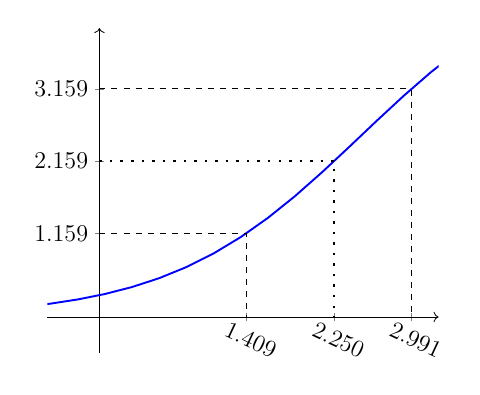
\begin{tikzpicture}[scale=0.725]
    \begin{axis}[
      axis lines=center,
      axis line style={->},
      xmin=-0.5, xmax=3.25,
      ymin=-0.5, ymax=4,
      xtick={1.409,2.25,2.991},
      xticklabels={1.409,2.250,2.991},
      ytick={1.159,2.159,3.159},
      yticklabels={1.159,2.159,3.159},
      xticklabel style={font=\large, rotate=-25, yshift=5pt},
      yticklabel style={font=\large},
      every axis plot/.append style={line width=0.95pt}
      ]
      \addplot[-] expression[domain=-1.25:5, blue] {5/(1+3^(2.5-x))};
      \draw[dashed] (axis cs: 0,1.159) -- (axis cs: 1.409,1.159) -- (axis cs: 1.409,0);
      \draw[dashed] (axis cs: 0,3.159) -- (axis cs: 2.991,3.159) -- (axis cs: 2.991,0);
      \draw[loosely dotted, line width=1.25pt] (axis cs: 0,2.159) -- (axis cs: 2.25,2.159) -- (axis cs: 2.25,0);
    \end{axis}
  \end{tikzpicture}
\end{flushright}
\vspace*{-15pt}
\pagebreak
\begin{ex*}
  Use the graph of $g(x)=\sqrt x+1$ to help find a number $\delta$ such that if $\abs{x-4}<\delta$ then $\ds\abs{\parens{\sqrt x+1}-3}<\frac{1}{2}$.
  \vspace*{-25pt}
  \begin{flushright}
    \begin{tikzpicture}
      \begin{axis}[
        axis lines=center,
        axis line style={->},
        xmin=-0.25, xmax=7.25,
        ymin=-0.25, ymax=4.5,
        xtick={2.25,4,6.25},
        xticklabels={$x_1$,4,$x_2$},
        ytick={2.5,3,3.5},
        ticklabel style={font=\large, inner sep=0.75pt},
        every axis plot/.append style={line width=0.95pt}
        ]
        \addplot[-] expression[blue, samples at={0,0.05,...,7.25}] {sqrt(x)+1};
        \draw[dashed] (axis cs: 0,2.5) -- (axis cs: 2.25,2.5) -- (axis cs: 2.25,0);
        \draw[dashed] (axis cs: 0,3.5) -- (axis cs: 6.25,3.5) -- (axis cs: 6.25,0);
        \draw[loosely dotted, line width=1.25pt] (axis cs: 0,3) -- (axis cs: 4,3) -- (axis cs: 4,0);
      \end{axis}
    \end{tikzpicture}
  \end{flushright}
\end{ex*}
\vspace{\stretch{1}}
\begin{ex*}
  Use the graph of the following linear function where $\ds\lim_{x \to 3} h(x)=5$ to find $\delta>0$ such that $\abs{h(x)-5}<1$ whenever $0<\abs{x-3}<\delta$.
  \begin{flushright}
    \begin{tikzpicture}
      \begin{axis}[
        axis lines=center,
        axis line style={->},
        grid=both,
        grid style={line width=0.35pt, draw=gray!75},
        xmin=-0.25, xmax=7.25,
        ymin=-0.25, ymax=7.25,
        xtick={0,1,...,7},
        ytick={0,1,...,7},
        ticklabel style={font=\large, inner sep=0.75pt},
        every axis plot/.append style={line width=0.95pt}
        ]
        \fill[color=ClemsonOrange, opacity=0.25] (axis cs:0,4) rectangle (axis cs: 8,6);
        \draw[dashed] (axis cs: 0,4) -- (axis cs: 8,4);
        \draw[dashed] (axis cs: 0,6) -- (axis cs: 8,6);
        \addplot[-] expression[blue, domain=-0.25:7.25] {0.5*x+3.5};
      \end{axis}
    \end{tikzpicture}
  \end{flushright}
\end{ex*}
\pagebreak
\noindent
\fbox{\parbox{\linewidth}{\textbf{Steps for proving that $\ds\lim_{x \to a} f(x)=L$}
  \begin{enumerate}
    \item \textbf{Find }$\bm \delta.$ Let $\eps$ be an arbitrary positive number. Use the inequality $\abs{f(x)-L}<\eps$ to find a condition of the form $\abs{x-a}<\delta$, where $\delta$ depends only on the value of $\eps$.
    \item \textbf{Write a proof.} For any $\eps>0$, assume $0<\abs{x-a}<\delta$ and use the relationship between $\eps$ and $\delta$ found in Step 1 to prove that $\abs{f(x)-L}<\eps$.
  \end{enumerate}
  }}
  
  \begin{ex*}
    Use the $\eps-\delta$ definition of a limit to prove $\ds\lim_{x \to 4}(2x-5)=3$.
    \vspace*{\stretch{1}}
  \end{ex*}
  \begin{ex*}
    Use the $\eps-\delta$ definition of a limit to prove $\ds\lim_{x \to 2}\dfrac{x}{5}=\dfrac{2}{5}$.
    \vspace*{\stretch{1}}
  \end{ex*}
  \pagebreak
  \begin{ex*}
    Use the $\eps-\delta$ definition of a limit to prove $\ds\lim_{x \to 2}\dfrac{x^2+x-6}{x-2}=5$.
    \vspace*{\stretch{1}}
  \end{ex*}
  \begin{ex*}
    Use the $\eps-\delta$ definition of a limit to prove $\ds\lim_{x \to 3}\dfrac{x^2+2x-15}{2x-6}=4$.
    \vspace*{\stretch{1}}
  \end{ex*}
  \pagebreak
\end{document}

\input{briggs3_01}
\input{briggs3_02}
\input{briggs3_03}
\input{briggs3_04}
\input{briggs3_05}
\input{briggs3_06}
\documentclass[answers]{exam}
\usepackage{texPreamble}
\usepackage{relsize}
\usepackage{tabularx}
\extraheadheight{0.25in}
\extrafootheight{1.0in}
\extrawidth{1in}
% ----------------------------------------------------------------
\firstpagefootrule
\runningfootrule
\begin{document}
%\relscale{1.4}
\section{3.7: The Chain Rule}
\begin{center}
  \fbox{\parbox{0.95\linewidth}{
    \textbf{Theorem 3.13} The Chain Rule
    
    Suppose $y=f(u)$ is differentiable at $u=g(x)$ and $u=g(x)$ is differentiable at $x$. The composite function $y=f(g(x))$ is differentiable at $x$, and its derivative can be expressed in two equivalent ways.
      \begin{align}
        &\dfrac{dy}{dx} = \dfrac{dy}{du}\cdot \dfrac{du}{dx}\\[10pt]
        &\dfrac{d}{dx}\parens{f\parens{g(x)}}=f'\parens{g(x)}\cdot g'(x)
      \end{align}
  }}
\end{center}
\begin{ex*}
  Take the derivatives of the following functions
\end{ex*}
\begin{tasks}[after-item-skip=\stretch{1}](2)
  \task $y=\parens{3x^3+1}^2$
  \task $y=\parens{3x^3+1}^7$
  \task $y=6\cos^2(x)$
  \task $y=\sin\parens{x+\cot(x)}$
\end{tasks}
\vspace*{\stretch{1}}
\begin{center}
  \fbox{\parbox{0.95\linewidth}{
    To use the chain rule,
    \begin{itemize}
      \item Identify the inner and outer function
      \item Take the derivative of the outside, leaving the original inner function
      \item Multiply by the derivative of the inner function
    \end{itemize}
  }}
\end{center}
\pagebreak

\begin{tasks}[resume, after-item-skip=\stretch{1}](2)
  \task $y(x)=e\inv[4x]$
  \task $y(x)=\parens{\dfrac{x-2}{2x+1}}^9$
  \task $y(x)=\sqrt{\sec(x)}$
  \task $y(x)=2\parens{8x-1}^3$
  \task $y(x)=\parens{\frac{x}{2}-1}\inv[10]$
  \task $y(t)=e^{\sin(t)}+\sin(e^t)$
\end{tasks}
\vspace*{\stretch{1}}
\pagebreak

\begin{tasks}[resume, after-item-skip=\stretch{1}](2)
  \task $y(x)=x^2 e^{x^2}$
  \task $\dfrac{f(x)}{g(x)}=f(x)\cdot\sbrkt{g(x)}\inv$
  \task $y(x)=f\parens{g\parens{h(x)}}$
  \task $y(x)=-12e^{3x^7}$
  \task* $y(x)=\dfrac{\cos^2(x)}{e^x\parens{x^2+4}}$
  
\end{tasks}
\vspace*{\stretch{1}}
\pagebreak

\end{document}

\documentclass[answers]{exam}
\usepackage{texPreamble}
\usepackage{relsize}
\usepackage{tabularx}
\extraheadheight{0.25in}
\extrafootheight{1.0in}
\extrawidth{1in}
% ----------------------------------------------------------------
\firstpagefootrule
\runningfootrule
\begin{document}
%\relscale{1.4}

\section{3.8: Implicit Differentiation}
Up until now, we have only taken the derivatives of \textit{explicitly} defined functions (functions defined in terms of only $x$). 

\noindent
An \textit{implicitly} defined function will be written in terms of both $x$ and $y$:
  $$x^2+y^2=25$$
\begin{center}
  \begin{tikzpicture}
    \begin{groupplot}[
      group style={group size=2 by 1},
      axis equal,
      axis lines=center,
      axis line style={->},
      ymin=-6.5, ymax=6.5,
      xtick={-5,5},
      ytick={-5,5},
      ticklabel style={font=\large, inner sep=0.75pt,fill=white},
      every axis plot/.append style={line width=0.95pt}, 
      samples=251, domain=-5:5,
      ]
      \nextgroupplot
        \addplot[-] expression[black]{sqrt(25-x^2)} node at (4.45,5.8) {$x^2+y^2=25$};
        \addplot[-] expression[black]{-sqrt(25-x^2)};
      \nextgroupplot
        \addplot[-] expression[ClemsonPurple]{sqrt(25-x^2)} node[black] at (4.1,5.8) {$y=\sqrt{25-x^2}$};
        \addplot[-] expression[ClemsonOrange]{-sqrt(25-x^2)} node[black] at (4.1,-5.5) {$y=-\sqrt{25-x^2}$};
    \end{groupplot}
  \end{tikzpicture}
\vfill 
  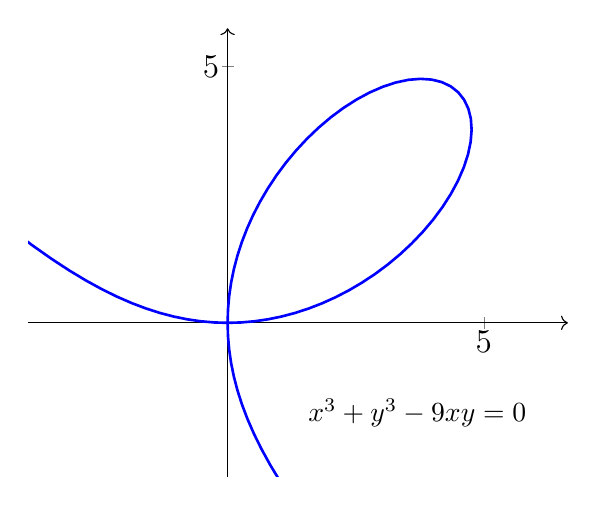
\begin{tikzpicture}
    \begin{axis}[
      axis equal,
      axis lines=center,
      axis line style={->},
      xmin=-3, xmax=5.75,
      ymin=-3, ymax=5.75,
      xtick={-5,5},
      ytick={-5,5},
      ticklabel style={font=\large, inner sep=0.75pt,fill=white},
      ]
      \draw[samples=100,domain=125:-40, line width=0.95pt, blue] plot(\x:{9*sin(\x)*cos(\x)/(sin(\x)^3+cos(\x)^3)}) node[black] at (3.7,-1.75) {$x^3+y^3-9xy=0$};
    \end{axis}
  \end{tikzpicture}
\vfill 
\end{center}
\pagebreak

\begin{center}\fbox{\parbox{0.7\linewidth}{

\textbf{Implicit Differentiation:}
  \begin{enumerate}
    \item Differentiate both sides of the equation with respect to $x$, treating $y$ as a differentiable function of $x$.
    \item Collect the terms with $\sfrac{dy}{dx}$ on one side of the equation.
    \item Solve for $\sfrac{dy}{dx}$.
  \end{enumerate}
}}\end{center}

\begin{ex*}
  Find the derivatives of the following by rewriting each function explicitly before taking the derivative, and by using implicit differentiation. Compare the results.
\end{ex*}

\begin{enumerate}[label=, itemsep=\stretch{1}]
  \item $y^2=x$
  \item $\sqrt x+\sqrt y=4$
\end{enumerate}
\vfill 
\pagebreak
\begin{ex*}
  Find the derivatives of the following equations:
\end{ex*}

\begin{tasks}[after-item-skip=\stretch{1}, label=~](2)
  \task $x^2+y^2=25$
  \task $x^3+y^3-9xy=0$
  \task $2y=x^2+\sin y$
  \task $x^2y^2+x\sin y=4$
  \task $y^5+x^2y^3=1+x^4y$
  \task $1+x=\sin\parens{xy^2}$
\end{tasks}
\vfill
\pagebreak

\begin{ex*}
  Find the derivatives of the following equations:
\end{ex*}
\begin{tasks}[after-item-skip=\stretch{1}, label=~](2)
  \task $x^3-xy+y^3=1$
  \task $xe^y=x-y$
  \task $\dfrac{1}{x}+\dfrac{1}{y}=1$
  \task $x^2-2x^3y^4+y^2=30y$
  \task $\tan(xy)=x+y$
  \task $x^2=\dfrac{x-y}{x+y}$
\end{tasks}
\vfill
\pagebreak

\begin{ex*}
  Find the second derivative implicitly for the following equations:
\end{ex*}
\begin{tasks}[after-item-skip=\stretch{1}, label=~](1)
  \task $y^2-2x=1-2y$
  \task $xy=\cot(xy)$
  \task $x^3+y^3=1$
  \task $x=e^y$
\end{tasks}
\vfill
\pagebreak

\begin{ex*}
  Find the equation of all lines tangent to the curve $x+y^3-y=1$ at $x=1$.
\end{ex*}
\vfill
%% This royal PITA needs to be compiled using 
%% shell-escape since it uses gnuplot
%%%%% pdflatex -shell-escape impFunc.tex %%%%%
\includegraphics[width=0.4\linewidth]{impFunc1}

\begin{ex*}
  Find the equation of the tangent line and normal line for $\parens{x^2+y^2-2x}^2=2\parens{x^2+y^2}$ at $(x,y)=(2,2)$.  
\end{ex*}
\vfill
\includegraphics[width=0.4\linewidth]{impFunc2}

\pagebreak

\end{document}

\input{briggs3_09}
\input{briggs3_10}
\input{briggs3_11}
\documentclass[answers]{exam}
\usepackage{texPreamble}
\usepackage{relsize}
\usepackage{tabularx}
\extraheadheight{0.25in}
\extrafootheight{1.0in}
\extrawidth{1in}
% ----------------------------------------------------------------
\firstpagefootrule
\runningfootrule
\begin{document}
%\relscale{1.4}
\section{4.1: Maxima and Minima}
\begin{defn*}[Absolute Maximum and Minimum]
  Let $f$ be defined on a set $D$ containing $c$. 
  \begin{itemize}
    \item 
      If $f(c)\geq f(x)$ for every $x$ in $D$, then $f(c)$ is an \textbf{absolute maximum} value of $f$ on $D$.
    \item 
      If $f(c)\leq f(x)$ for every $x$ in $D$, then $f(c)$ is an \textbf{absolute minimum} value of $f$ on $D$.
    \item 
      An \textbf{absolute extreme value} is either an absolute maximum value or an absolute minimum value.
  \end{itemize}
\end{defn*}
\vspace*{\stretch{1}}
\begin{ex*}
  Determine whether the function has any absolute extreme values
\end{ex*}
\begin{center}
  \begin{tikzpicture}
    \begin{groupplot}[
      group style={group size=3 by 2, horizontal sep=2cm, vertical sep=2cm},
      axis lines=center,
      axis line style={->},
      width=0.3\linewidth,
      ticklabel style={font=\footnotesize,inner sep=0.5pt,fill=white,opacity=1.0, text opacity=1},
      xlabel=$x$, xlabel style={at={(ticklabel* cs:1)},anchor=north west},
      ylabel=$y$, ylabel style={at={(ticklabel* cs:1)},anchor=south},
      every axis plot/.append style={line width=0.95pt, color=blue}
      ]
      \nextgroupplot[
        xmin=-6, xmax=6,
        ymin=-6, ymax=6,
        ylabel=${y=-x^2+4}$, 
        ]
        \addplot[<->] expression[domain=-3:3]{-x^2+4};
      \nextgroupplot[
        xmin=-6, xmax=6,
        ymin=-6, ymax=6,
        ylabel=${y=\frac{x^3}{3}+x^2+1}$,
        ]
        \addplot[<->] expression[domain=-4.125:1.775]{x^3/3+x^2+1};
      \nextgroupplot[
        xmin=-6.75, xmax=6.75,
        ymin=-1.5, ymax=1.5,
        ylabel=${y=\sin(x)}$,
        xtick={-6.28318, -3.141592, ..., 6.28318},
        xticklabels={$-2\pi$,$-\pi$, ,$\pi$, $2\pi$},
        ]
        \addplot[<->] expression[domain=-6.0:6.0, samples=100]{sin(deg(x))};
      \nextgroupplot[
        xmin=-4.5, xmax=4.5,
        ymin=-2, ymax=8.5,
        ylabel=${y=x^2-1}$ on ${[-3,2]}$,
        ]
        \addplot[-] expression[domain=-3:2]{x^2-1};
        \addplot[soldot] coordinates{(-3,8)(2,3)};
      \nextgroupplot[
        xmin=-4.5, xmax=4.5,
        ymin=-2, ymax=8.5,
        ylabel=${y=x^2-1}$ on ${[-3,2)}$,
        ]
        \addplot[-] expression[domain=-3:2]{x^2-1};
        \addplot[holdot] coordinates{(2,3)};
        \addplot[soldot] coordinates{(-3,8)};
      \nextgroupplot[
        xmin=-4.5, xmax=4.5,
        ymin=-2, ymax=8.5,
        ylabel=${y=x^2-1}$ on ${(-3,2)}$,
        ]
        \addplot[-] expression[domain=-3:2]{x^2-1};
        \addplot[holdot] coordinates{(-3,8)(2,3)};
    \end{groupplot}
  \end{tikzpicture}
\end{center}
\vspace*{\stretch{1}}
\pagebreak

\noindent
\fbox{\parbox{0.9875\linewidth}{\textbf{Theorem 4.1: Extreme Value Theorem}

A function that is continuous on a closed interval $\sbrkt{a,b}$ has an absolute maximum value and an absolute minimum value on that interval.
}}

\begin{center}
  \begin{tikzpicture}
    \begin{groupplot}[
      group style={group size=3 by 1, horizontal sep=1.5cm},
      axis lines=center,
      width=0.35\linewidth,
      axis line style={->},
      ticklabel style={font=\footnotesize,inner sep=0.5pt,fill=white,opacity=1.0, text opacity=1},
      xlabel=$x$, xlabel style={at={(ticklabel* cs:1)},anchor=north west},
      ylabel=$y$, ylabel style={at={(ticklabel* cs:1)},anchor=south west},
      every axis plot/.append style={line width=0.95pt, color=blue}
      ]
      \nextgroupplot[
        xmin=-2.5, xmax=3.5,
        ymin=-4.75, ymax=6.25,
        ] 
        \addplot[-] expression[domain=-1.075:3, samples=100]{(x-1)*(x-2)*(x+1)*x*(x-3)+2};
      \nextgroupplot[
        xmin=-2.5, xmax=3.5,
        ymin=-4.5, ymax=6.25,
        ] 
        \addplot[-] expression[domain=-1.075:3, samples=100]{(x-0.5)^2-3};
        \addplot[soldot] coordinates{(-1.075,-0.519375)(3,3.25)};
      \nextgroupplot[
        xmin=-2.5, xmax=3.5,
        ymin=-4.75, ymax=6.25,
        ] 
        \addplot[-] expression[samples=100]{2};
        \addplot[soldot] coordinates{(-2.5,2)(3.5,2)};
    \end{groupplot}
  \end{tikzpicture}
\end{center}
\vspace*{\stretch{1}}
\textit{Note:} It is important that the function is both continuous \textit{and} the interval is closed:
\begin{center}
  \begin{tikzpicture}
    \begin{groupplot}[
      group style={group size=2 by 1, horizontal sep=1.5cm},
      axis lines=center,
      width=0.35\linewidth,
      axis line style={->},
      ticklabel style={font=\footnotesize,inner sep=0.5pt,fill=white,opacity=1.0, text opacity=1},
      xlabel=$x$, xlabel style={at={(ticklabel* cs:1)},anchor=north west},
      ylabel=$y$, ylabel style={at={(ticklabel* cs:1)},anchor=south west},
      every axis plot/.append style={line width=0.95pt, color=blue}
      ]
      \nextgroupplot[
        xmin=0, xmax=3.75,
        ymin=0, ymax=3.75,
        ]
        \addplot[-] expression[domain=1:2]{(x-1)^2+1};
        \addplot[-] expression[domain=2:3, samples=100]{sqrt(3-x)+1.25};
        \addplot[soldot] coordinates{(1,1)(2,2)(3,1.25)};
        \addplot[holdot] coordinates{(2,2.25)};
      \nextgroupplot[
        xmin=-0.5, xmax=2.5,
        ymin=-0.5, ymax=10,
        ymajorticks=false,
        ]
        \addplot[-] expression[domain=0:1.9, samples=100]{1/(2-x)+1/2};
        \draw[densely dashed] (2,-0.5)--(2,10);
        \addplot[holdot] coordinates{(0,1)};
    \end{groupplot}
  \end{tikzpicture}
\end{center}
\vspace*{\stretch{1}}
\pagebreak

\begin{defn*}[Local Maximum and Minimum Values]
  Suppose $c$ is an interior point of some interval $I$ on which $f$ is defined. If $f(c)\geq f(x)$ for all $x$ in $I$, then $f(c)$ is a \textbf{local maximum} value of $f$. If $f(c)\leq f(x)$ for all $x$ in $I$, then $f(c)$ is a \textbf{local minimum value of $f$.}
\end{defn*}

\begin{center}
  \includegraphics[width=0.55\linewidth]{images/briggs_04_01/fig4_5.png}
\end{center}

\textit{Note:} Local extrema \textbf{CANNOT} occur at endpoints. 

\vspace*{\stretch{1}}
\begin{ex*}
  State the absolute extrema and the local extrema:
\end{ex*}
\begin{center}
  \begin{tikzpicture}
    \begin{groupplot}[
      group style={group size=3 by 2, horizontal sep=1.5cm, vertical sep=1.5cm},
      axis lines=center,
      width=0.325\linewidth,
      axis line style={->},
      ticklabel style={font=\normalsize,inner sep=0.5pt,fill=white,opacity=1.0, text opacity=1},
      xlabel=$x$, xlabel style={at={(ticklabel* cs:1)},anchor=north west},
      ylabel=$y$, ylabel style={at={(ticklabel* cs:1)},anchor=south west},
      every axis plot/.append style={line width=0.95pt, color=blue}
      ]
      \nextgroupplot[
        xmin=1.75, xmax=6,
        ymin=0, ymax=6,
        xtick={2.384,3.506,4.704,5.75},
        xticklabels={$a$, $c_1$, $c_2$, $b$},
        ymajorticks=false,
        ]
        \addplot[-] expression[domain=2.384:5.75, samples=100]{(x-2)*(x-3)*(x-4)*(x-5.125)+2};
        \addplot[soldot] coordinates{(2.384,0.9522)(5.45,6)};
      \nextgroupplot[
        xmin=1.75, xmax=6,
        ymin=0, ymax=3,
        xtick={2.5,4,5.5},
        xticklabels={$a$, $c_1$, $b$},
        ymajorticks=false,
        ]
        \addplot[-] expression[domain=2.5:4,samples=501]{-(4-x)/abs(4-x)*abs(4-x)^(1/3)+2};
        \addplot[-] expression[domain=4:5.5,samples=501]{(4-x)/abs(4-x)*abs(4-x)^(1/3)+2};
        \addplot[holdot] coordinates{(2.5,0.85)(5.5,0.85)};
      \nextgroupplot[
        xmin=-3.5, xmax=2.5,
        ymin=-1.5, ymax=2.5,
        ]
        \addplot[-] expression[domain=-3:0]{-x/3-1};
        \addplot[-] expression[domain=0:1]{3*x-1};
        \addplot[-] expression[domain=1:2]{-2*x+4};
        \addplot[soldot] coordinates{(-3,0)(0,-1)(1,2)(2,0)};
    \end{groupplot}
  \end{tikzpicture}
\end{center}
\vspace*{\stretch{1}}
\pagebreak

\begin{ex*}
  Sketch the graph of a continuous function $f$ on $\sbrkt{0,4}$ satisfying the given properties:
\end{ex*}

\begin{enumerate}
  \item 
    $f'(x)=0$ for $x=1,2$ and $3$; $f$ has an absolute minimum at $x=1$; $f$ has no local extremum at $x=2$; and $f$ has an absolute maximum at $x=3$.

    \begin{tikzpicture}
      \begin{axis}[
        axis lines=center,
        axis line style={->},
        xmin=-0.5, xmax=4.5,
        ymin=-6, ymax=6,
        xtick={-6,-5,...,6},
        height=2.24in,
        width=\linewidth,
        ymajorticks=false,
        ticklabel style={font=\small,inner sep=0.5pt,fill=white,opacity=1.0, text opacity=1},
        ]
      \end{axis}
    \end{tikzpicture}
  \item 
    $f'(1)$ and $f'(3)$ are undefined; $f'(2)=0$; $f$ has a local maximum at $x=1$; $f$ has a local minimum at $x=2$; $f$ has an absolute maximum at $x=3$; and $f$ has an absolute minimum at $x=4$.

    \begin{tikzpicture}
      \begin{axis}[
        axis lines=center,
        axis line style={->},
        xmin=-0.5, xmax=4.5,
        ymin=-6, ymax=6,
        xtick={-6,-5,...,6},
        height=2.24in,
        width=\linewidth,
        ymajorticks=false,
        ticklabel style={font=\small,inner sep=0.5pt,fill=white,opacity=1.0, text opacity=1},
        ]
      \end{axis}
    \end{tikzpicture}
  \item 
    $f'(x)=0$ at $x=1$ and $3$; $f'(2)$ is undefined; $f$ has an absolute maximum at $x=2$; $f$ has neither a local maximum nor a local minimum at $x=1$; and $f$ has an absolute minimum at $x=3$.

    \begin{tikzpicture}
      \begin{axis}[
        axis lines=center,
        axis line style={->},
        xmin=-0.5, xmax=4.5,
        ymin=-6, ymax=6,
        xtick={-6,-5,...,6},
        height=2.24in,
        width=\linewidth,
        ymajorticks=false,
        ticklabel style={font=\small,inner sep=0.5pt,fill=white,opacity=1.0, text opacity=1},
        ]
      \end{axis}
    \end{tikzpicture}
\end{enumerate}
%\vspace*{\stretch{1}}
\pagebreak

\noindent
\fbox{\parbox{0.9875\linewidth}{\textbf{Theorem 4.2: Local Extreme Value Theorem}
  
  If $f$ has a local maximum or minimum value at $c$ and $f'(c)$ exists, then $f'(c)=0$.
}}
\begin{center}
  \textit{Note:} If the derivative is zero, then the function \textbf{MIGHT} have a max/min.  
\end{center}

\begin{ex*}
  Sketch a graph of a function $f(x)$ that has a local maximum value at a point $c$ where $f'(c)$ is defined.
\end{ex*}
\vspace*{\stretch{1}}
\begin{ex*}
  Sketch a graph of a function $f(x)$ that has a local maximum value at a point $c$ where $f'(c)$ is undefined.
\end{ex*}
\vspace*{\stretch{1}}
\begin{ex*}
  Graph 
  \begin{tasks}(2)
    \task $f(x)=x^3$
    \task $f(x)=\abs{x}$
  \end{tasks}
\end{ex*}
\vspace*{\stretch{1}}
\pagebreak
\begin{defn*}[Critical Point]
  An interior point $c$ of the domain of $f$ at which $f'(c)=0$ \textit{or} $f'(c)$ fails to exist is called a \textbf{critical point} of $f$.
\end{defn*}
\begin{ex*}
  Find the critical points of
\end{ex*}
\begin{tasks}[after-item-skip=\stretch{1}, label=~](1)
  \task $f(x)=x^3+3x^2-24x$
  \task $g(x)=\sqrt{4-x^2}$
  \task $h(t)=3t-\sin\inv(t)$
\end{tasks}
\vspace*{\stretch{1}}
\pagebreak
\begin{ex*}
  Find the critical points of
\end{ex*}
\begin{tasks}[after-item-skip=\stretch{1}, label=~](1)
  \task $f(x)=\sin(x)\cos(x)$ on $\sbrkt{0,2\pi}$. 
  \task $f(t)=t^2-2\ln(t^2+1)$
  \task $f(x)=x\sqrt{x-a}$
  \task $f(x)=\sin\inv(x)\cos\inv(x)$
\end{tasks}
\vspace*{\stretch{1}}
\pagebreak
\begin{center}
  \fbox{\parbox{0.8\linewidth}{
    How to find the absolute max/min of $f(x)$ on $\sbrkt{a,b}$:
    \begin{enumerate}
      \item 
        Find $f'(x)$
      \item 
        Find all critical points ($f'(x)=0$ or $f'(x)$ \textbf{DNE})
      \item 
        Evaluate $f(x)$ at the critical points within $\sbrkt{a,b}$ and the end points.
      \item 
        Identify the absolute max and absolute min using the values found. Include value and location (e.g. ordered pair $(x,y)$)
    \end{enumerate}
    }}
\end{center}
\begin{ex*}
  Find the absolute max and min of $f(x)=2x-2x^\frac{2}{3}$ on $\sbrkt{-1,3}$.
\end{ex*}
\vspace*{\stretch{1}}

\begin{ex*}
  Find the absolute max and min of $f(x)=\frac{x}{x^2+1}$ on $\sbrkt{0,2}$.
\end{ex*}
\vspace*{\stretch{1}}

\begin{ex*}
  Find the absolute max and min of $f(x)=3x^4-4x^3-12x^2+1$ on $\sbrkt{-2,3}$.
\end{ex*}
\vspace*{\stretch{1}}
\pagebreak

\begin{ex*}
  Find the absolute max and min of $f(x)=\sin(3x)$ on $\sbrkt{-\frac{\pi}{4},\frac{\pi}{3}}$.
\end{ex*}
\vspace*{\stretch{1}}

\begin{ex*}
  Find the absolute max and min of $f(x)=xe^{1-\frac{x}{2}}$ on $\sbrkt{0,5}$.
\end{ex*}
\vspace*{\stretch{1}}

\begin{ex*}
  Find the absolute max and min of $f(x)=e^x-2x$ on $\sbrkt{0,2}$.
\end{ex*}
\vspace*{\stretch{1}}
\pagebreak

\begin{ex*}
  Find the absolute max and min of $f(x)=x^\frac{1}{3}(x+4)$ on $\sbrkt{-27,27}$.
\end{ex*}
\vspace*{\stretch{1}}

\begin{ex*}
  Find the absolute max and min of $y=\sqrt{x^2-1}$.
\end{ex*}
\vspace*{\stretch{1}}

\begin{ex*}
  Find the absolute/local max and min of $f(x)=x^2\parens{x^2+4x-8}$ on $\sbrkt{-5,2}$.
\end{ex*}
\vspace*{\stretch{1}}
\pagebreak

\begin{ex*}
  \textbf{Minimum-surface-area box} 
  %TODO Future Peter
  % S(x)=2x^2+\frac{4V}{x}
  
  All boxes with a square base of length $x$ and a volume $V$ have a surface area given by $S(x)=x^2+\frac{4V}{x}$. Find $x$ such that the box has volume $50\,ft^3$ with minimal surface area.
\end{ex*}
\vspace*{\stretch{1}}

\begin{ex*}
  \textbf{Trajectory high point}
  
  A stone is launched vertically upward from a cliff $192\,ft$ above the ground at a speed of $64\,ft/s$. Its height above the ground $t$ seconds after the launch is given by $s=-16t^2+64t+192,$ for $0\leq t\leq 6$. When does the stone reach its maximum height?
\end{ex*}
\vspace*{\stretch{1}}
\pagebreak

\begin{ex*}
  \textbf{Maximizing Revenue}
  
  A sales analyst determines that the revenue from sales of fruit smoothies is given by $R(x)=-60x^2+300x$, where $x$ is the price in dollars charged per item, for $0\leq x\leq 5$.
  \begin{enumerate}[label=\alph*)]
    \item 
      Find the critical points of the revenue function.
    \item 
      Determine the absolute maximum value of the revenue function and the price that maximizes the revenue.
  \end{enumerate}
\end{ex*}
\pagebreak

\begin{ex*}
  Find the absolute and local extreme values of the following
  \begin{enumerate}[itemsep=\stretch{1}]
    \item $f(x)=\abs{x-3}+\abs{x+2}$ on $\sbrkt{-4,4}$,
    \item $g(x)=\abs{x-3}-2\abs{x+1}$ on $\sbrkt{-2,3}$.
  \end{enumerate}
\end{ex*}
\vspace*{\stretch{1}}
\pagebreak

\begin{ex*}
  \textbf{Every second counts} (4.01: Q87)
  
  You must get from a point $P$ on the straight shore of a lake to a stranded swimmer who is $50\,m$ from a point $Q$ on the shore that is $50\,m$ from you. Assuming that you can swim at a speed of $2\,m/s$ and run at a speed of $4\,m/s$, the goal of this exercise is to determine the point along the shore, $x$ meters from $Q$, where should you stop running and start swimming to reach the swimmer in the minimum time.

\noindent
\begin{minipage}{0.675\linewidth}
  \begin{enumerate}[label=\alph*)]
    \item 
      Find the function $T$ that gives the travel time as a function of $x$, where $0\leq x\leq 50$.
    \item 
      Find the critical point of $T$ on $(0,50)$.
    \item 
      Evaluate $T$ at the critical point and the endpoints ($x=0$ and $x=50$) to verify that the critical point corresponds to an absolute minimum. What is the minimum travel time?
    \item 
      Graph the function $T$ to check your work.
  \end{enumerate}
\end{minipage}%
\begin{minipage}{0.325\linewidth}
  \begin{flushright}
    \includegraphics[width=0.95\linewidth]{images/briggs_04_01/swimming_q87.png}
  \end{flushright}
\end{minipage}~
\end{ex*}
\pagebreak

\end{document}

\input{briggs4_02}
\input{briggs4_03}
\input{briggs4_04}
\documentclass[answers]{exam}
\usepackage{texPreamble}
\usepackage{relsize}
\usepackage{tabularx}
\extraheadheight{0.25in}
\extrafootheight{1.0in}
\extrawidth{1in}
% ----------------------------------------------------------------
\firstpagefootrule
\runningfootrule
\begin{document}
%\relscale{1.4}
\section{4.6: Linear Approximation and Differentials}
\begin{ex*}
  Find the equation of the line tangent to $y=1+\sin(x)$ at $a=0$. State the line in the slope--intercept form.
\end{ex*}
\vspace*{\stretch{1}}
\begin{flushright}
  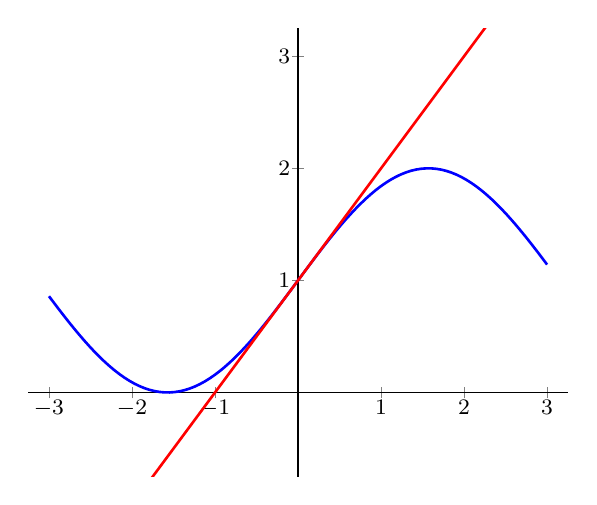
\begin{tikzpicture}
    \begin{axis}[
      grid style={line width=0.35pt, draw=gray!75},
      axis lines=center,
      axis line style={-},
      xmin=-3.25, xmax=3.25,
      ymin=-0.75, ymax=3.25,
      xtick={-6,-5,...,6},
      ytick={-6,-5,...,6},
      ticklabel style={font=\footnotesize,inner sep=0.5pt,fill=white,opacity=1.0, text opacity=1},
      every axis plot/.append style={line width=0.95pt, color=blue, samples=100}
      ]
      \addplot[-] expression[domain=-3:3]{1+sin(deg(x))};
      \addplot[-] expression[red]{x+1};
    \end{axis}
  \end{tikzpicture}
\end{flushright}
\begin{defn*}
  \textbf{Linear Approximation of $f$ at $a$.}
  
  Suppose $f$ if differentiable on an interval $I$ containing the point $a$. The \textbf{linear approximation} to $f$ at $a$ is the linear function.
  
  $$L(x)=f(a)+f'(a)(x-a),\ \textnormal{ for } x \textnormal{ in } I.$$
\end{defn*}
\pagebreak

\begin{ex*}
  Consider the function $f(x)=\dfrac{x}{x+1}$. Find the linearization at $a=1$. Use the linearization to estimate $f(1.1)$ and compare with the true value of $f(1.1)$.
\end{ex*}
\pagebreak

\begin{ex*}
  Find the linearization $L(x)$ of $f(x)=e^{3x-6}$ at $a=2$.
\end{ex*}
\vspace*{\stretch{1}}

\begin{ex*}
  Find the linearization $L(x)$ of $f(x)=9\parens{4x+11}^\frac{2}{3}$ at $a=4$.
\end{ex*}
\vspace*{\stretch{1}}

\begin{ex*}
  Find a linearization over an interval which will contain the given point $x_0$. Choose your center at a point \textit{near} $x_0$ but not at $x_0$ so that the given function and its derivative are easy to evaluate. Lastly, use the linearization to approximate $f(x_0)$.
\end{ex*}
\begin{enumerate}[label=\alph*), itemsep=\stretch{1}]
  \item $f(x)=x^2+2x,\ x_0=0.1$
  \item $f(x)=\sqrt[3]{x},\ x_0=8.5$.
\end{enumerate}
\vspace*{\stretch{1}}
\pagebreak

\begin{ex*}
  Use a linear approximation to estimate $\sqrt{146}$.
\end{ex*}
\vspace*{\stretch{1}}

\begin{ex*}
  Use a linear approximation to estimate $\parens{1.999}^4$.
\end{ex*}
\vspace*{\stretch{1}}

\begin{ex*}
  Use a linear approximation to estimate $\sqrt{\dfrac{5}{29}}$.
\end{ex*}
\vspace*{\stretch{1}}
\pagebreak

\begin{ex*}
  Find the linearization $L(x)$ of $f(x)=\sqrt{x^2+9}$ at $a=-4$. Use $L(x)$ to estimate $f(-4.1)$ and $\sqrt{23.44}$.
\end{ex*}
\vspace*{\stretch{1}}
\pagebreak

\begin{ex*}
  Use a linearization to show that $0.05$ is a good approximation for $\ln(1.05)$.
\end{ex*}
\pagebreak

\begin{ex*}
  Find the linearization of the following functions at the given point and use concavity to identify if the linearization is an overestimate or an underestimate.
\end{ex*}
\begin{enumerate}[label=\alph*),itemsep=\stretch{1}]
  \item $f(x)=\dfrac{2}{x};\, a=1$
  \item $f(x)=e\inv[x];\, a=\ln(2)$
\end{enumerate}
\vspace*{\stretch{1}}


\noindent
\fbox{\parbox{0.9875\linewidth}{
  \textbf{Summary: Uses of Linear Approximation}
  \begin{enumerate}
    \item 
      To approximate $f$ near $x=a$, use
        $$f(x)\approx L(x)=f(a)+f'(a)(x-a).$$
    \item 
      To approximate the change $\Delta y$ in the dependent variable when the independent variable $x$ changes from $a$ to $a+\Delta x$, use
        $$\Delta y\approx f'(a)\Delta x.$$
  \end{enumerate}
}}
\pagebreak

\begin{defn*}[Differentials]
  
  Let $f$ be differentiable on an interval containing $x$. A small change in $x$ is denoted by the \textbf{differential} $dx$. The corresponding change in $f$ is approximated by the \textbf{differential} $dy=f'(x)\,dx$. So if $\Delta x=dx$, where $\Delta x$ and $dx$ are both small, then $\Delta y\approx dy$:
    \[\Delta y= f(x+dx)-f(x)\approx dy=f'(x)\,dx.\]
    
\end{defn*}

\begin{ex*}
  Find the differential $dy$.
\end{ex*}
\begin{tasks}[after-item-skip=\stretch{1}, label=~](2)
  \task $y=\cos(x^2)$
  \task $y=\sqrt{1-x^2}$
  \task $y=4x^2-3x+2$
  \task $y=x\tan(x^3)$
  \task $y=\cos^5(x)$
  \task $f(x)=\sin\inv(x)$
\end{tasks}
\vspace*{\stretch{1}}
\pagebreak
\begin{ex*}
  Let $y=x^2$
\end{ex*}
\begin{enumerate}[label=\alph*), itemsep=\stretch{1}]
  \item Find $dy$
  \item If $x=1$ and $dx=0.01$, find $dy$.
  \item Compare $dy$ and $\Delta y$ at this point.
\end{enumerate}
\vspace*{\stretch{1}}

\begin{ex*}
  Let $y=\sqrt{3+x^2}$
\end{ex*}
\begin{enumerate}[label=\alph*), itemsep=\stretch{1}]
  \item Find $dy$
  \item If $x=1$ and $dx=-0.1$, find $dy$.
  \item Compare $dy$ and $\Delta y$ at this point.
\end{enumerate}
\vspace*{\stretch{1}}

\pagebreak
\begin{ex*}
  Suppose $f$ is differentiable on $(-\infty,\infty)$ and $f(5.01)-f(5)=0.25$. Use linear approximation to estimate the value of $f'(5)$.
\end{ex*}
\vspace*{\stretch{1}}

\begin{ex*}
  Suppose $f$ is differentiable on $(-\infty,\infty)$ and $f(5.99)=7$ and $f(6)=7.002$. Use linear approximation to estimate the value of $f'(6)$.
\end{ex*}
\vspace*{\stretch{1}}
\pagebreak

\begin{ex*}
  Compute $dy$ and $\Delta y$ for $y=e^x$ when $x=0$ and $\Delta x=0.5$.
\end{ex*}
\vspace*{\stretch{1}}

\begin{ex*}
  Approximate the change in the area of a circle when its radius increases from $2.00$ to $2.02\,m$.
\end{ex*}
\vspace*{\stretch{1}}

\begin{ex*}
  Approximate the change in the magnitude of the electrostatic force between two charges when the distance between them increases from $r=20\,m$ to $r=21\,m$ $(F(r)=0.01/r^2$).
\end{ex*}
\vspace*{\stretch{1}}
\pagebreak

\begin{ex*}
  Approximate the change in the volume of a right circular cylinder of fixed radius $r=20\,cm$ when its height decreases from $h=12\,cm$ to $h=11.9\,cm$ ($V(h)=\pi r^2h$).
\end{ex*}
\vspace*{\stretch{1}}

\begin{ex*}
  Approximate the change in the volume of a right circular cylinder of a right circular cone of fixed height $h=4\,m$ when its radius increases from $r=3\,m$ to $r=3.05\,m$ ($V(r)=\frac{1}{3}\pi r^2 h$).
\end{ex*}
\vspace*{\stretch{1}}
\pagebreak

\begin{ex*}
  The radius of a sphere is measured and found to be $0.7$ inches with a possible error in measurement of at most 0.01 inches.
\end{ex*}
\begin{enumerate}[label=\alph*), itemsep=\stretch{1}]
  \item What is the maximum error in using the value of the radius to compute the volume of the sphere?
  \item Find the relative error of the volume: \hfill\textit{relative error} $\dfrac{dV}{V}$\hspace*{50pt}
  
  What is the percentage error?
\end{enumerate}
\vspace*{\stretch{1}}
\pagebreak

\begin{ex*}
  The radius of a circular disk is given as $24\,cm$ with a maximum error in measurement of $0.2\,cm$.
\end{ex*}
\begin{enumerate}[label=\alph*), itemsep=\stretch{1}]
  \item Use differentials to estimate the maximum error in the calculated area of the disk.
  \item What is the relative error? What is the percentage error?
\end{enumerate}
\vspace*{\stretch{1}}
\pagebreak

\begin{ex*}
  Use differentials to estimate the amount of paint needed to apply a coat of paint $0.05\,cm$ thick to a hemispherical dome with diameter $50\,m$.
\end{ex*}
\vspace*{\stretch{1}}
\pagebreak
\end{document}

\input{briggs4_07}
\input{briggs4_05}
\input{briggs4_09}
\input{briggs5_01}
\input{briggs5_02}
\input{briggs5_03}
\documentclass[answers]{exam}
\usepackage{texPreamble}
\usepackage{relsize}
\usepackage{tabularx}
\extraheadheight{0.25in}
\extrafootheight{1.0in}
\extrawidth{1in}
% ----------------------------------------------------------------
\firstpagefootrule
\runningfootrule
\begin{document}
%\relscale{1.4}
\section{5.4: Working with Integrals}

\fbox{\parbox{0.9875\linewidth}{
  \textbf{Theorem 5.4: Integrals of Even and Odd Functions}
  
  Let $a$ be a positive real number and let $f$ be an integrable function on the interval $\sbrkt{-a,a}$.
  \begin{itemize}
    \item If $f$ is even, $\ds\int_{-a}^a f(x)\,dx=2\int_{0}^a f(x)\,dx.$
    \item If $f$ is odd, $\ds\int_{-a}^a f(x)\,dx=0.$
  \end{itemize}
}}

\begin{ex*}
  Rewrite the following trig functions to determine if it is even or odd:
  \begin{tasks}[label=\mbox{}](2)
    \task $\sin(-x)=$
    \task $\cos(-x)=$
    \task $\tan(-x)=$
    \task $\cot(-x)=$
    \task $\csc(-x)=$
    \task $\sec(-x)=$
  \end{tasks}
  Use this to rewrite and evaluate the following integrals:
\end{ex*}
\begin{tasks}[after-item-skip=\stretch{1}, label=\mbox{}](2)
  \task $\ds\int_{-\pi}^\pi \sin(x)\,dx$
  \task $\ds\int_{-\pi}^\pi \cos(x)\,dx$
  \task $\ds\int_{-\pi/4}^{\pi/4} \tan(x)\,dx$
  \task $\ds\int_{-\pi/4}^{\pi/4} \sec(x)\,dx$
\end{tasks}
\vspace*{\stretch{1}}
\textit{Note:} $\cot(x)$ and $\csc(x)$ are excluded here as they are not continuous on $\sbrkt{-\frac{\pi}{4},\frac{\pi}{4}}$.

\vspace*{-\baselineskip}
\pagebreak

\begin{ex*}
  Use symmetry to evaluate the following integrals:
\end{ex*}
\begin{tasks}[after-item-skip=\stretch{1}](1)
  \task $\ds\int_{-10}^{10} \frac{x}{\sqrt{200-x^2}}\,dx$
  \task $\ds\int_{-2}^{2}\parens{x^9-3x^5+2x^2-10}\,dx$
\end{tasks}
\vspace*{\stretch{1}}
\pagebreak

\begin{tasks}[after-item-skip=\stretch{1}, resume](1)
  \task $\ds\int_{-\frac{\pi}{4}}^{\frac{\pi}{4}}\sin^5(x)\,dx$
  \task $\ds\int_{-1}^{1}\parens{1-\abs{x}}\,dx$
  \task $\ds\int_{-2}^{2}\frac{x^3-4x}{x^2+1}\,dx$
\end{tasks}
\vspace*{\stretch{1}}
\pagebreak

\begin{ex*}
  Given that $f(x)$ is even and $\ds\int_{-8}^{8} f(x)\,dx=18$, find
\end{ex*}
\begin{tasks}(2)
  \task $\ds\int_{0}^{8}f(x)\,dx$
  \task $\ds\int_{-8}^{8}xf(x)\,dx$
\end{tasks}
\vspace*{\stretch{1}}
\begin{ex*}
  Given that $f(x)$ is odd and $\ds\int_{0}^{4} f(x)\,dx=3$ and $\ds\int_0^8 f(x)\,dx=9$, find
\end{ex*}
\begin{tasks}(2)
  \task $\ds\int_{-4}^{8}f(x)\,dx$
  \task $\ds\int_{-8}^{4}f(x)\,dx$
\end{tasks}
\vspace*{\stretch{1}}
\pagebreak

\begin{ex*}
  Use symmetry to explain why
\end{ex*}
  \[\int_{-4}^{4}\parens{5x^4+3x^3+2x^2+x+1}\,dx=2\int_0^4 \parens{5x^4+2x^2+1}\,dx\]

  \vspace*{\stretch{1}}
\begin{ex*}
  Evaluate
\end{ex*}
  $\ds\int_{-\frac{\pi}{2}}^{\frac{\pi}{2}}\parens{\cos(2\theta)+\cos(\theta)\sin(\theta)-3\sin(\theta^5)}\,d\theta$
\vspace*{\stretch{1}}
\begin{ex*}
  While the following integrals are not on symmetric intervals, symmetry still applies here:
\end{ex*}
\begin{tasks}(3)
  \task $\ds\int_0^\pi \cos(x)\,dx$
  \task $\ds\int_0^{2\pi} \sin(x)\,dx$
  \task $\ds\int_0^{4\pi} \cos(x)\,dx$
\end{tasks}
\vspace*{\stretch{1}}
\pagebreak

\begin{defn*}[Average Value of a Function]
  The average value of an integrable function $f$ on the interval $\sbrkt{a,b}$ is
    \[\bar f= \frac{1}{b-a}\int_a^b f(x)\,dx.\]
\end{defn*}
\begin{ex*}
  Find the average value of $f(x)=-\dfrac{x^2}{2}$ on $\sbrkt{0,3}$.
\end{ex*}
\vspace*{\stretch{1}}
\begin{ex*}
  Find the average value of $f(x)=3x^2-3$ on $\sbrkt{0,1}$.
\end{ex*}
\vspace*{\stretch{1}}
\begin{ex*}
  Find the average value of $f(t)=t^2-t$ on $\sbrkt{-2,1}$.
\end{ex*}
\vspace*{\stretch{1}}
\pagebreak

\begin{ex*}
  Find the average value of $f(x)=\dfrac{1}{x^2+1}$ on $\sbrkt{-1,1}$.
\end{ex*}
\vspace*{\stretch{1}}
\begin{ex*}
  Find the average value of $f(x)=\dfrac{1}{x}$ on $\sbrkt{1,e}$.
\end{ex*}
\vspace*{\stretch{1}}
\begin{ex*}
  Find the average value of $f(x)=x^\frac{1}{n}$ on $\sbrkt{0,1}$.
\end{ex*}
\vspace*{\stretch{1}}
\pagebreak

\begin{ex*}
  The velocity in $m/s$ of an object moving along a line over the time interval $\sbrkt{0,6}$ is $v(t)=t^2+3t$. Find the average velocity of the object over this time interval.
\end{ex*}
\vspace*{\stretch{1}}

\begin{ex*}
  A rock is launched vertically upward from the ground with a speed of $64 ft/s$. The height of the rock (in $ft$) above the ground after $t$ seconds is given by the function $s(t)=-16t^2+64t$. Find its average velocity during its flight.
\end{ex*}
\vspace*{\stretch{1}}

\pagebreak
\begin{ex*}
  The surface of a water wave is described by $y=5\parens{1+\cos(x)}$, for $-\pi\leq x\leq \pi$, where $y=0$ corresponds to a trough of the wave. Find the average height of the wave above the trough on $\sbrkt{-\pi,\pi}$.
\end{ex*}

\noindent
\begin{minipage}{0.5\linewidth}
  \begin{tikzpicture}
    \begin{axis}[
      axis lines=center,
      axis line style={->},
      xmin=-1.2*pi, xmax=1.2*pi,
      ymin=-0.5, ymax=11,
      height=2.5in, width=3.5in,
      xtick={-3.141592654,-1.570796327,1.570796327,3.141592654},
      xticklabels={$-\pi$,$-\sfrac{\pi}{2}$,$\sfrac{\pi}{2}$,$\pi$},
      ticklabel style={font=\small,inner sep=0.5pt,fill=white,opacity=1.0, text opacity=1},
      xlabel=$x$, xlabel style={at={(ticklabel* cs:1)},anchor=north west},
      ylabel=$y$, ylabel style={at={(ticklabel* cs:1)},anchor=south west},
      every axis plot/.append style={line width=0.95pt, color=blue, samples=100}
      ]
      \addplot[-] expression[domain=-pi:pi] {5*(1+cos(x*180/pi))};
    \end{axis}
  \end{tikzpicture}
\end{minipage}
\pagebreak

\noindent
\fbox{\parbox{0.9875\linewidth}{
  \textbf{Theorem 5.5: Mean Value Theorem for Integrals}

  Let $f$ be continuous on the interval $\sbrkt{a,b}$. There exists a point $c$ in $\parens{a,b}$ such that 
    \[f(c)=\bar f=\frac{1}{b-a}\int_a^b f(t)\,dt\]
}}
\begin{ex*}
  For the following problems, find the point(s) that satisfy the Mean Value Theorem for Integrals.
\end{ex*}
\begin{tasks}[after-item-skip=\stretch{1}](1)
  \task $f(x)=\dfrac{1}{x^2}$ on $\sbrkt{1,4}$.
  \task $f(x)=e^x$ on $\sbrkt{0,2}$.
  \task $f(x)=\cos(x)$ on $\sbrkt{-\dfrac{\pi}{2},\dfrac{\pi}{2}}$
  \task $f(x)=1-\abs{x}$ on $\sbrkt{-1,1}$.
\end{tasks}
\vspace*{\stretch{1}}

%TODO remove relscale
\pagebreak
\end{document}

\input{briggs5_05}
\end{document}
